\chapter{Radio Foregrounds and Rotation Measure Synthesis} % Main chapter title

\label{Chapter3} % For referencing the chapter elsewhere, use \ref{Chapter1} 

\textbf{Overview}\\
% \HRule \\[0.4cm]
\par\noindent\rule{\textwidth}{0.4pt}\\
\textit{This chapter presents a brief theoretical review of the diffuse synchrotron emis-
sion and Faraday rotation. We then discuss the simulation algorithm used to
produce the foreground maps with rotation in this research.}
\par\noindent\rule{\textwidth}{0.4pt}\\
% --------------------------------------------------------------------------------------------------------------------------------

%\lhead{Chapter 3. \emph{Cosmological Signal}}


% \HRule \\[1.5cm]
% --------------------------------------------------------------------------------------------------------------------------------
\noindent \texttt{Author’s comment}: 
%%
\small{Part of this work is taken from: \textbf{T. Ansah-Narh}, F. B. Abdalla, O. M. Smirnov, K. M. B. Asad and J. R. Shaw, (2018). Simulations of Systematic Direction-dependent Instrumental Effects in Intensity Mapping Experiments. Monthly Notices of the Royal Astronomical Society (MNRAS), published. It is therefore, widely recognized that some of the text and figures will match that of the article. Therefore, this comment serves as a general reference for all such text.
}

\section{Galactic Foreground}	   \label{chap3:sec1}
%% 
% \texttt{Author’s comment: The indentation part in this section is taken from the work of} \citep{ansah2018simulations}.
% A varying magnetic field can accelerate charge particles to emit radiation.
The measurements of redshifted CO and 21 cm emissions are very powerful tools to understand the star formation and survey the structure of the Universe respectively. 
The emission emerging from different astrophysical sources, other than the signals mentioned above, results in the foreground emission whose magnitude can be the higher than
fourth order of the expected signals. The EM emission from particles normally electrons accelerated by the death of a star and supernova remnant, in the presence of a magnetic field, 
is called the \emph{synchrotron emission}. The synchrotron emission from the Galaxy dominates at low microwave frequencies $(\lesssim 30 \, \rm GHz)$, 
whilst that of thermal dust emission is at higher frequencies $(\gtrsim 70 \, \rm GHz)$. Between these two components in frequency, lies the thermal free-free and non-thermal 
dust emissions, which are formed as a result of spinning dust grains \citep{2016A&A...594A..10P} as shown in Fig.~\ref{fig:cmb1}. 
The free-free emission (also known as thermal bremsstrahlung) is obtained from thermally hot electrons ($\gtrsim 10^4\, \rm K$) \citep{1999astro.ph..2201S} scattering uniformly in
the interstellar plasma hence, having a completely zero polarisation. In the case of the thermal dust emission,
it is formed from dust grains that get warmed by the interstellar radiation field and then emit far-infrared light which eventually lead to multiple temperatures.
The dust grains are composed of Polycyclic Aromatic Hydrocarbons (PAHs), silicates, and graphites. 


%	+++++++++++++++++++++++++++++++++++++++++++
%	Foreground Emission
%	++++++++++++++++++++++++++++++++++++++++++++
%
\begin{figure}[ht]
	    \centering	    
	    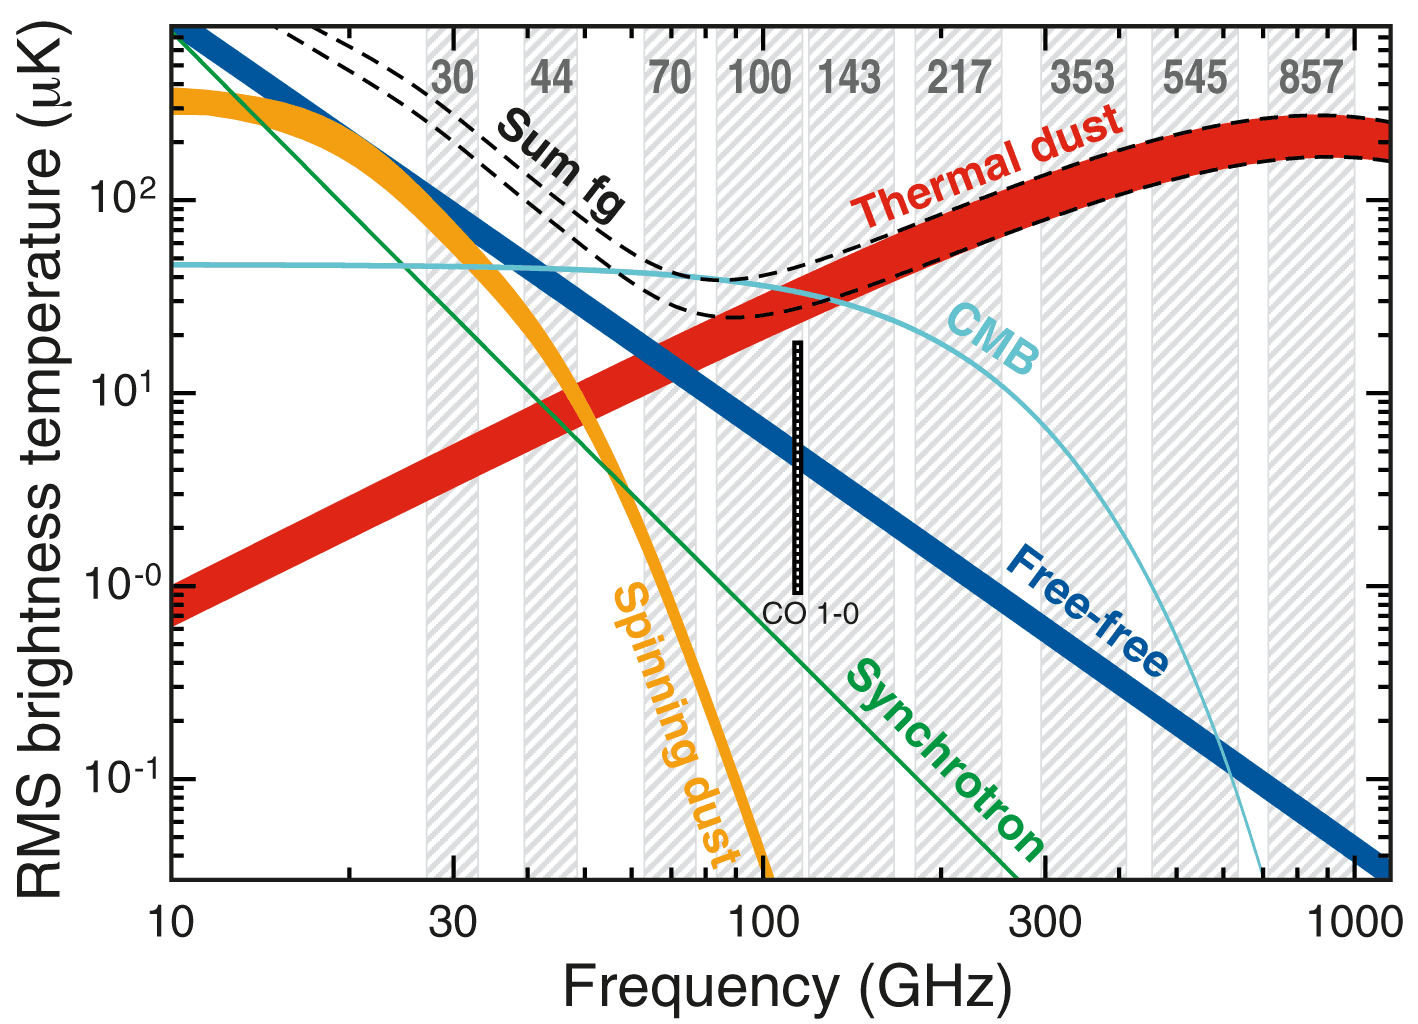
\includegraphics[width=3.8in]{c3/Planck_A12_Fig24_left} %cmb1}	    	   
	    \caption{\theo{Brightness temperature distribution for the components of the Galactic foregrounds with respect to frequency. 
	    The angular resolution for the temperature of each smooth component is $1^\circ$.
	    \emph{Credit:} This figure is obtained from \citep{2016A&A...594A..10P}.}} \label{fig:cmb1}
% 	    {\textit{A model of radio galaxy spectrum \citep[see][]{Murphy:2010kk}. The individual contributions from non-thermal synchrotron, 
% 	    free-free, and thermal dust emission are indicated by dot-dashed, triple dot-dashed, and dashed lines, respectively.} }	   
       \end{figure}
  \FloatBarrier  

\noindent Detailed discussion of the components of the Galactic foregrounds, paying particular attention to their contributions to the polarization
measurements can be found in \cite{2015MNRAS.447..400A,2010MNRAS.409.1647J,2015aska.confE..19S,2014MNRAS.441.3271W}.
% }
% \citep{ansah2018simulations}
% \end{quotation}
 %%
%%


%
\subsection{Diffuse Galactic Synchrotron Emission}	   \label{chap3:sec2.1}
%

 
% A varying magnetic field can accelerate charge particles to emit radiation.
% Galactic synchrotron radiation occurs when the interstellar  magnetic field interacts with charged particles (electrons and positrons) in the cosmic-ray.
% These interacting particles are accelerated to relativistic speeds in very high energetic environments,
% such as shock-waves from supernovae explosions. The synchrotron intensity and spectrum depend on the magnetic field strength and cosmic ray energy,
% showing significant spatial variations on the sky. The energy distribution of cosmic ray electrons follows a power-law 
\theo{
In Section~\ref{chap3:sec1}, we emphasized that the intensity of the synchrotron radiation relies on the strength of the magnetic field and the cosmic-ray energy. 
The distribution of this energy can be given as a function of a power law (also known as scaling law) such that $N_{\rm \,E} \varpropto E^{-\tau}$, where 
$E > 10$ GeV is the energy \citep{2011PhRvL.106t1101A} and $\tau \approx 3.0 $ is the spectral index  of the energy distribution (this index value is usually accepted when modelling
in synchrotron and magnetic field). }
%%

\theo{The intensity of a synchrotron radiation $S_{\rm \, sync}$ with a frequency $\nu$ is defined as \citep{MD2008}: 
% %
\begin{equation}  \label{eq:th1}
  S_{\rm \,  sync}(\nu) = \varepsilon_{\rm \, sync}(\nu)\, \int\limits_z \, n_{\rm \, e}B_{\rm \, \perp}^{(1+\tau)/2}\, dz   
 \end{equation} 
% 
}
\theo{where Equation~\ref{eq:th1} is integrated with respect to the sight-line $z$, $n_{\rm \, e}$ is cosmic ray density and 
$B_{\rm \, \perp} = \sqrt{B_{\rm \, x}^{2} + B_{\rm \, y}^{2}}$ is the $x,y$  components of the magnetic field of the sky.
From the power law, we can express the emissivity term $ \varepsilon_{\rm \, sync}(\nu)$ as:
 %
\begin{equation}
 \varepsilon_{\rm \, sync}(\nu) = \varepsilon_{\rm \, 0}\, \nu^{-(\tau - 1)/2}
 \label{eq:th2}
 \end{equation} 
 %
}
\theo{Recall Rayleigh-Jeans law at frequency $\nu$:
 %
\begin{equation}
  B_{\rm \, \nu}(T) = \frac{2\nu^{2}k_{\rm \, B}T}{c^2}
  \label{eq:th3}
 \end{equation} 
 %
 where $c$ denotes the speed of light, $k_{\rm \, B}$ being the Boltzmann constant and $T$ is the temperature in Kelvin. Using Equation~\ref{eq:th3}, 
 we can convert Equation~\ref{eq:th1} into a brightness temperature $T_{\rm \, sync}$ at frequency $\nu$:
 %
\begin{equation}
  T_{\rm \, sync}(\nu) = \frac{c^{2}S_{\rm \, sync}(\nu)}{2k_{\rm \, B}\nu^2}
  \label{eq:th4}
 \end{equation} 
 %
} 
 \theo{Hence, expressing $T_{\rm \, sync}$ as a power law, we get:
 %
\begin{equation}
  T_{\rm \, sync}(\nu) = T_{\rm \, sync}(\nu_0)\left(\frac{\nu}{\nu_0}\right)^{\gamma_{\rm \, sync}}
  \label{eq:th5}
 \end{equation} 
 %
 where $\gamma_{\rm \, sync} = -(\tau + 3)/2$. The spectral index $\gamma_{\rm \, sync}$, changes at  different frequency bands as displayed in Table~\ref{table:2}.}
 %
%

\begin{table}[H]
\caption{Measured Spectral Indices at Different Frequency Bands}             % title of Table
\label{table:2}      % is used to refer this table in the text
%\begin{threeparttable}
\centering                          % used for centering table
\begin{tabular}{c c}        	  % centered columns (4 columns)
\hline\hline                	  % inserts double horizontal lines
\textbf{$\gamma_{\rm \, sync}$} & \textbf{Frequency Band ($\rm GHz$)}\\    % table heading 
   %
\hline                        % inserts single horizontal line
  $-2.55$ & $0.045 - 0.408$ \\      % inserting body of the table
  $-2.71$ & $0.408 - 2.30$ \\
  $-3.01$ & $2.300 - 33.0$ \\  
\hline                                   %inserts single line
\end{tabular}
% 
\end{table}
 \FloatBarrier 
\theo{
\noindent Fig.~\ref{fig:ch3.3} is the $408$ MHz full-sky survey taken from the LAMBDA-Data Products\footnote{ 
\url{https://lambda.gsfc.nasa.gov/product/foreground/fg_2014_haslam_408_info.cfm}} \citep{2015MNRAS.451.4311R} and originally produced by \citep{1981A&A...100..209H,HaslamMap} 
displaying the sky in mollview form in Galactic  coordinates at a frequency where the diffuse synchrotron emission is most dominant. We can clearly observe other sources 
 outside the Milky Way such as Cen A galaxy and the Magellanic clouds. An in-depth explanation on the concept of synchrotron emission is conferred in \citep{lightman1979radiative}.
}
 %
%	+++++++++++++++++++++++++++++++++++++++++++
%	full-sky map
%	++++++++++++++++++++++++++++++++++++++++++++
%
\begin{figure}[ht]
	    \centering	    
	    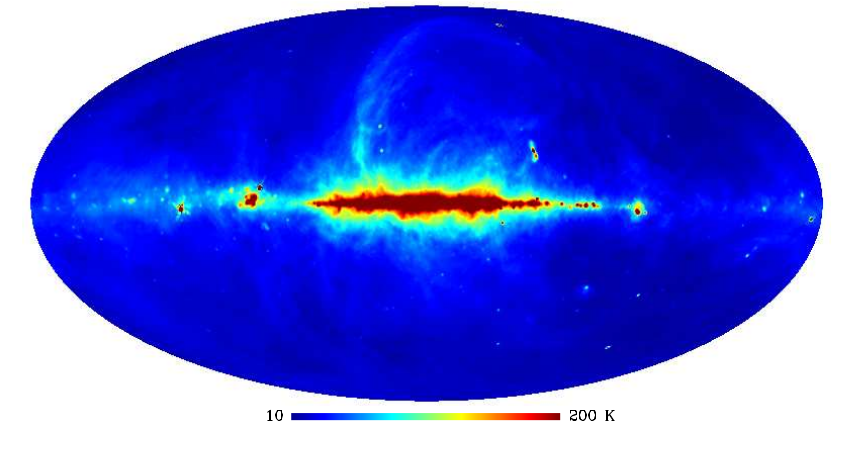
\includegraphics[width=3.8in]{c3/haslam}	    	   
	    \caption{$408$ MHz Full-Sky Map \citep{1981A&A...100..209H} projected in HEALPix, ring
and defined in Galactic coordinates. Data and images can be retrieved from the LAMBDA website.}
	    \label{fig:ch3.3}
       \end{figure}
  \FloatBarrier   
  %
\theo{
\noindent However, studies such as \citep{2010MNRAS.409.1647J,2018ApJ...855...29H} have shown that generally, the diffuse Galactic synchrotron emission is incompletely 
linearly polarised. This is due to the \enquote{spatial and energy distribution of the cosmic ray electrons, as well as the strength and orientation of 
the perpendicular (with respect to the line of sight) component of the Galactic
magnetic field} \citep{2010MNRAS.409.1647J}. Note that the distribution of charge particles can alter smoothly with  pitch angle and this can eliminate the circular part and hence, 
become partially linearly polarised. Therefore, using the cosmic rays and magnetic field distributions of a galaxy, we can predict 
the polarisation foreground from the synchrotron emission and then separate it from observed maps.
The degree of linear polarisation integrated over all electron energy and frequency 
is computed as $l = (\tau + 1)/(\tau + 7/3)$\citep{2010MNRAS.409.1647J,lightman1979radiative}. The polarisation factor ($l$) can be increased to $0.75$ if 
the cosmic ray spectral index $\tau \approx 3$. We can express the polarised intensity in terms of Stokes parameters $Q$ and $U$ at frequency $\nu$ such that:
}
%
\theo{
\begin{equation}
  \begin{aligned}
  lI_{\rm \nu} = \sqrt{Q_{\rm \nu}^2 + U_{\rm \nu}^2}
   \end{aligned}
%    \phantom{\hspace{1cm}}
  \label{eq:th6}
 \end{equation} 
 %%
\noindent with the angle of polarisation given as:
%
%
\begin{equation}
  \begin{aligned}
  \varphi_{\rm \nu} = \frac{1}{2}\arctan \left( \frac{U_{\rm \nu}}{Q_{\rm \nu}} \right)
   \end{aligned}
%    \phantom{\hspace{1cm}}
  \label{eq:th7}
 \end{equation} 
 %
Therefore, in the $Q,\, U$ plane, the modulus of the complex linear polarisation is computed as ($\lvert Q_{\rm \nu} + jU_{\rm \nu} \rvert$).
From Equation~\ref{eq:th1}, we can integrate the polarised parameters ($Q$ and $U$) along the sight-line $z$ as \citep{MD2008}:
%
%
 %
\begin{equation}
  \begin{aligned}
  Q_{\rm \, sync}(\nu) = l_{\rm \, sync}\varepsilon_{\rm \, sync}(\nu)\, \int\limits_z \, n_{\rm \, e}B_{\rm \, \perp}^{(1+\tau)/2} \cos(2\alpha)\sin(\beta)\, dz
  \end{aligned}
%    \phantom{\hspace{1cm}}
  \label{eq:th8}
 \end{equation} 
 % 
%
and 
%
%
 %
\begin{equation}
  \begin{aligned}
  U_{\rm \, sync}(\nu) = l_{\rm \, sync}\varepsilon_{\rm \, sync}(\nu)\, \int\limits_z \, n_{\rm \, e}B_{\rm \, \perp}^{(1+\tau)/2} \sin(2\alpha)\sin(\beta)\, dz
  \end{aligned}
%    \phantom{\hspace{1cm}}
  \label{eq:th9}
 \end{equation} 
%
\noindent where $\cos(2\alpha) = \frac{B_x^2 - B_y^2}{B_{\rm \, \perp}^2} \quad 0 < \cos(2\alpha) < 1 $,\\
$\sin(2\alpha) = -\frac{B_x^2B_y^2}{B_{\rm \, \perp}^2}  \quad 0 < \sin(2\alpha)< 1$ and 
$\sin(\beta) = \sqrt{1 -\frac{B_x^2}{B_{\rm \, \perp}^2}}  \quad 0 < \sin(\beta) < 1$.
}


\section{Faraday Rotation Measure Synthesis}	    \label{chap3:Faraday}
%%
% \emph{Polarisation} is the term used to describe the orientation of the electric field in a light wave.
Usually, light is not polarized when created but can be made so by transporting it through a medium which transmits electric fields oriented in a specific direction and absorbs all others. 
Radio emission from astronomical sources, such as galactic and extra-galactic sources and pulsars is often linearly polarized. Of course, other sources such as OH masers from galactic star formation due to Zeeman splitting 
are mostly circularly polarized \citep{2008ApJ...680..981R}. Generally, polarization in radio astronomy is related to the presence of magnetic fields. 
For instance, radio emission due to synchrotron radiation is linearly polarized with the electric vectors and it is directed at right angles to the magnetic field in the line of emission 
onto the sky plane \citep{2012A&A...540A..80B}. However, the polarization direction may alter as the radio waves
propagate through the ISM. This effect is called the Faraday rotation and it allows radio astronomers to understand the magnetic field strength in the line-of-sight for both ISM and
Earth's ionosphere.
%heiles2008zeeman

The degree of polarization of Faraday rotation is quantified in terms of it's rotation measure ($\Phi_{\rm \, RM}$) and it is mathematically expressed as;
%%
\begin{equation}\label{eq:pangle}
\chi(\lambda) = \chi_{\rm \, 0} + \Phi_{\rm \, RM}.\lambda^2 
\end{equation}

such that, 
 \begin{equation}\label{eq:rm}
  \Phi_{\rm \, RM} = 0.81 \int_{\rm \, source}^{observer} n_{\rm \, e} \vec{B}.d \vec{l}	
 \end{equation}
%\overrightarrow{B}

\noindent where the polarization angle measured at wavelength $\lambda$ is $\chi(\lambda)$, $\chi_{\rm \, 0}$ is the intrinsic polarization,
$n_{\rm \, e}$ is the density electron in cm\textsuperscript{-3}, $\mathbf{B}$ in $\mu$G describes the magnetic field  and $l$ in pc denotes the length of path.
 $\vec{B}.d \vec{l}$ describe the direction of the magnetic field along the sight line.
%%


The observed complex polarization is described by \citep{1966MNRAS.133...67B} as $P(\lambda^2) = pI\exp(2j\chi)$, where $p$ is the degree of polarization. Substituting 
Equation~\ref{eq:pangle} for $\chi$ in \citep{1966MNRAS.133...67B} equation and integrating over all possible values of the rotation measure to get;

 \begin{subequations}\label{eq:sub}
 \begin{align}
  P(\lambda^2) &=\, \int_{\rm \, - \infty}^{+ \infty} pI\exp(2j[\chi_{\rm \, 0} + \Phi_{\rm \, RM}.\lambda^2 ]) d\Phi_{\rm \, RM} \label{eq:suba}\\
               &=\, \int_{\rm \, - \infty}^{+ \infty} F(\Phi_{\rm \, RM})\exp(2j\Phi_{\rm \, RM}.\lambda^2) d\Phi_{\rm \, RM} \label{eq:subb}
  \end{align}
 \end{subequations}
%%
where the intrinsic polarized flux is characterised by the \emph{Faraday dispersion function} $F(\Phi_{\rm \, RM})$ in terms of Faraday depth.
Note how the expression in Equation~\ref{eq:subb} takes the form of a Fourier transform. Therefore, we can invert Equation~\ref{eq:subb}  to obtain the intrinsic
polarization in terms of observable quantities to have;
%%
\begin{equation}\label{eq:invert}
F(\Phi_{\rm \, RM}) = \int_{\rm \, - \infty}^{+ \infty} P(\lambda^2)\exp(-2j\Phi_{\rm \, RM}.\lambda^2) d\lambda^2
\end{equation}
%%

% \noindent  \citep{2005A&A...441.1217B} proposed a window function $W(\lambda^2)$ to address the situations where we cannot observe at wavelengths $\lambda^2 < 0 $ 
% nor observe at all values of $\lambda^2 > 0 $.
%%

In the next section, we present how to simulate the polarized sky maps used in this research and account for the Faraday rotation. 

%% 

 \section{Simulation}    \label{sec:simulation}
%%
We apply the \texttt{CORA} software package\footnote{{\url{https://github.com/radiocosmology/cora/}}} \citep{shaw2015coaxing,Shaw:2013} to reproduce the 
complete polarization sky maps at different frequencies as shown in Figs.~\ref{fig:f1000} to~\ref{fig:f1306}. Even though the foreground simulations
are produced in a scheme similar to those described in \cite{shaw2015coaxing}, we have significantly expanded the description in this work to make it more self contained. 
% 

As now described in \citep{ansah2018simulations}, the polarization sector is simulated by generating a distribution of polarized emission in Faraday space. 
This is designed to make simulations sufficiently complex in the spectral direction, roughly reproduce the polarized 
amplitude across the sky, but does not attempt to match polarization angles anywhere. In addition, the spectral structure of the polarized signal 
from the galaxy occurs because the emission is from a range of Faraday depths. 
As suggested, the 3D structure of the galaxy, particularly the magnetic field means that emission from different regions along the 
line-of-sight collect varying amounts of Faraday rotation. In general, this gives complicated frequency dependent polarized structure 
with multiple independent Faraday components \citep[see Figure 9]{wolleben2010rotation}. Accurate mapping of this distribution is difficult, 
but is being attempted by projects such as GMIMS\footnote{{Global Magneto-Ionic Medium Survey}} \citep{GMIMS}. The most useful full-sky 
polarization measurements come from $1.4$ GHz surveys \citep{Wolleben2006,Testori2008}, the WMAP $23$ GHz \citep{WMAP_9yr_maps},
and Planck $30$ GHz maps \citep{Planck_2015_maps}. However, because of the uncertain amount of instrumental depolarization in the former and the much 
higher frequencies of the latter, these are more useful to tell us about the general properties of the polarized sky (such as the high galactic latitude
polarization fraction, see \cite{Kogut2007}) and less about the specific realisation on the sky.
Due to these drawbacks, the level of polarization within the galactic plane produced in the simulations is appropriate for IM experiments.  %\\~\\
%%
\begin{figure}[ht]
	    \centering
	    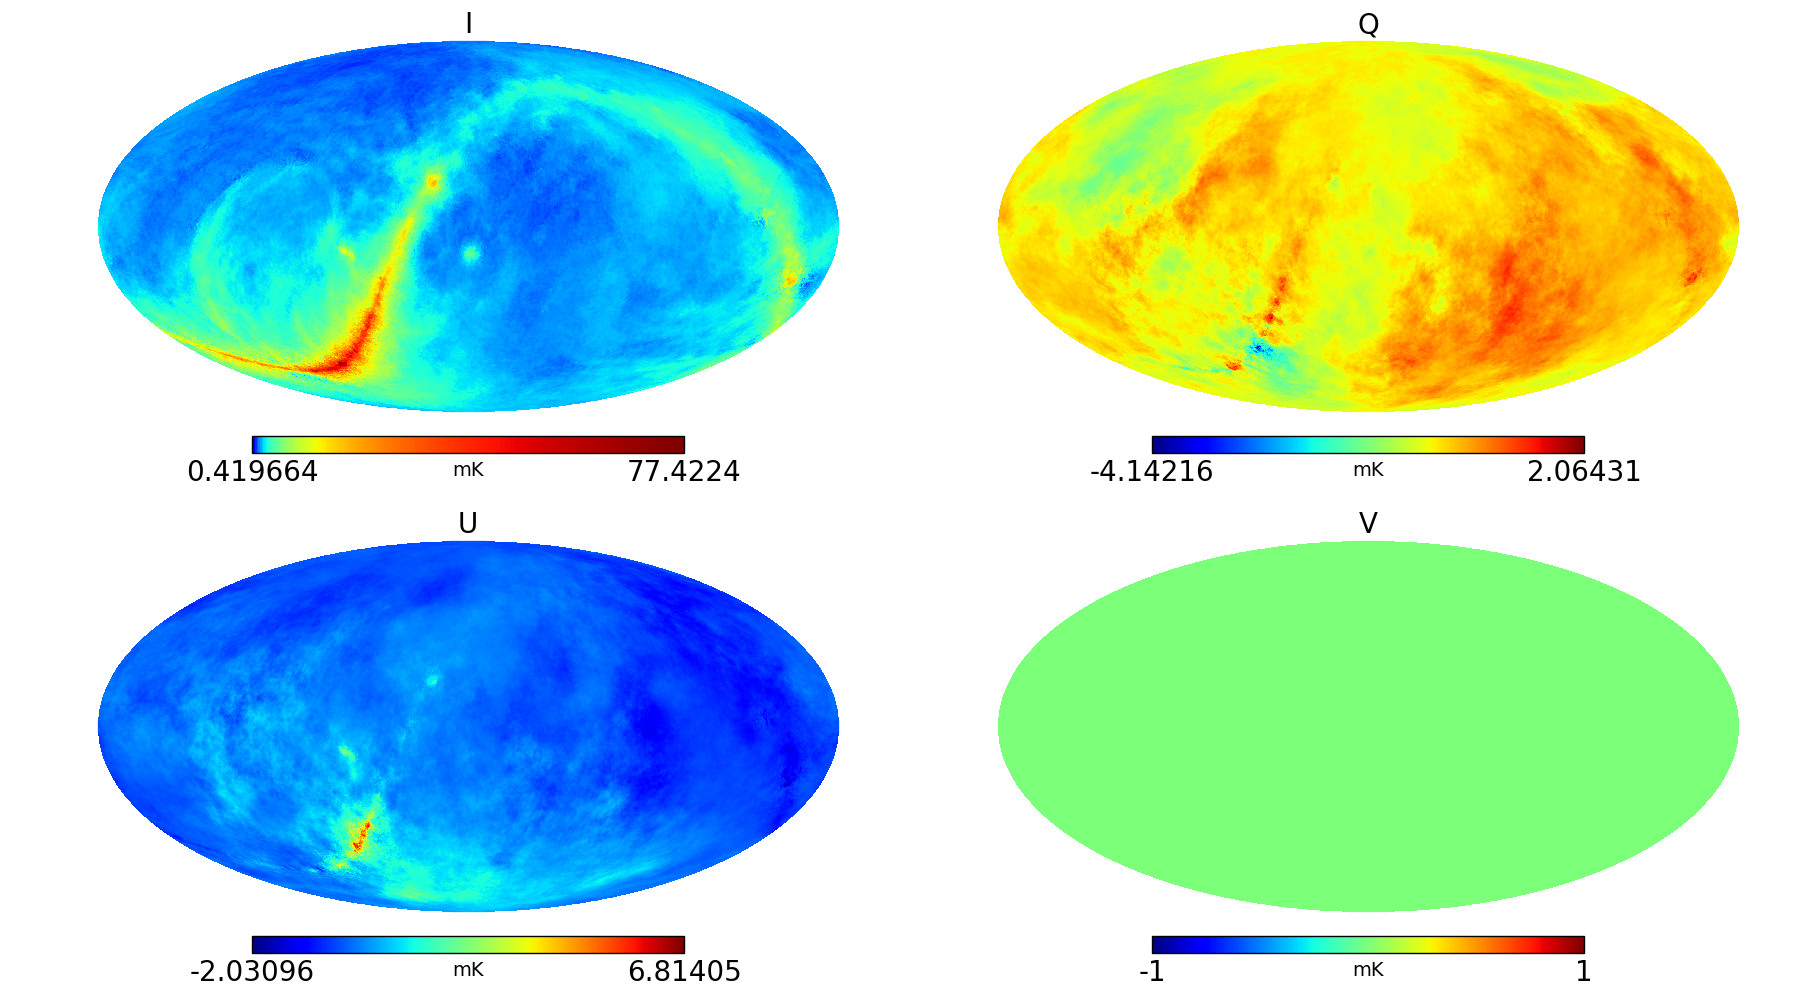
\includegraphics[width=6.0in]{c4/sec3gp_conv/Tchan_253}
	    \caption{1000 MHz full-sky simulated synchrotron maps. These synchrotron maps characterize the 
     full-sky polarization maps for our low resolution simulated observations and are presented here in the mollweide projection form defined by equatorial coordinates in terms of Stokes parameters $I, Q, U$ and $V$.}
	    \label{fig:f1000}
       \end{figure}
\FloatBarrier

Below is the scheme used to generate the foreground simulations:

\begin{enumerate}[label=(\roman*)]
 \item A 3D base map for the unpolarized sky is produced by extrapolating the $408$ MHz \cite{HaslamMap} map to the requested set of frequencies using 
    the spectral index of map of \cite{MD2008} which     was produced by comparing the Haslam map with WMAP $23$ GHz polarization data, assuming that both are dominated by 
    synchrotron emission. This produces a map with power law spectral behaviour with angular fluctuations on scales $\gtrsim 1^\circ$ scales.

    \item Angular and spectral fluctuations are added into the 3D maps according to an angular power spectrum.
    \begin{equation}
        C_\ell(\nu, \nu') \propto \biggl(\frac{\ell}{\ell_0}\biggr)^{-2.8} \biggl(\frac{\nu \nu'}{\nu_0^2}\biggr)^{-2.8} \exp{\Biggl[- \frac{1}{2} \biggl(\frac{\ln{\nu / \nu'}}{4}\biggr)^2\Biggr]} \; ,
    \end{equation}
    taken from \cite{SantosCoorayKnox}. We use a position dependent scaling on large scales to ensure the fluctuations to match their observed variance across the sky
    \citep{LaPorta2008},
    and ensure that we don't add in additional fluctuations on scales constrained by the Haslam map by projecting out the the dominant eigenmodes on these scales.

    \item To simulate the polarized sky, we use the ideas of Faraday Rotation Measure Synthesis \citep{Brentjens2005} and a simple model of the distribution of emission in 
    Faraday depth across the full sky, which we then integrate over to generate the polarized output at each desired frequency. To produce the emission in Faraday space, 
    we use the rotation 
    measure map of \cite{Oppermann2012} to indicate the characteristic scale of the distribution of emission in Faraday depth. We tune the amplitude and correlation 
    properties in Faraday 
    space to crudely reproduce the polarization fraction in the WMAP $23$ GHz map and the $1.4$ GHz surveys. The polarization directions are generated as 
    a Gaussian random field at each
    Faraday depth. For the interested reader, more details of this are found in  \cite{shaw2015coaxing}.

    \item Known bright point sources on the sky are included explicitly, with their polarizations Faraday rotated to the desired frequencies using the \cite{Oppermann2012} map. 
    Faint sources ($S < 10$ Jy at $151$ MHz) are randomly generated.
\end{enumerate} 


Finally, we use the \enquote{Hierarchical Equal Area isoLatitude Pixelation} (\texttt{HEALPix}\footnote{\url{http://healpix.sourceforge.net/}}) 
software \citep{calabretta2007mapping,2005ApJ...622..759G} to project the simulated full-sky maps
into equal pixel area, using a resolution of $N_{\rm \, \rm s} = 512$. This makes our gridded map to uniformly distribute $12N_{\rm \, \rm s}^2$ pixels onto a unit sphere. 
The regular synchrotron maps in Figs.~\ref{fig:f1000} to~\ref{fig:f1306} are depicted in  \texttt{HEALPix} format at different frequencies. 


%  
%  \begin{figure}[H]{\columnwidth}
%       \centering      
%       \includegraphics[width=\linewidth]{/c5/mkk/m/mk_fraw1}         
%      \caption{$950$ MHz full-sky synchrotron maps simulated by using m-mode formalism.}
% 	    \label{fig:fgc5}    
%     \end{figure}
\begin{figure}[ht]
	    \centering
	    \includegraphics[width=6.0in]{c5/mkk/m/mk_fraw1} 
	    \caption{Simulated foreground maps at 950 MHz displayed in mollweide form.}
	    \label{fig:f950}
       \end{figure}
\FloatBarrier
%    
%   \begin{figure}[H]{\columnwidth}
%       \centering      
%       \includegraphics[width=\linewidth]{/c6/spatial/fb1}        
%      \caption{$450$ MHz full-sky synchrotron maps simulated by using m-mode formalism.}
% 	    \label{fig:fgc6B1}    
%     \end{figure}
   \begin{figure}[ht]
	    \centering
	    \includegraphics[width=6.0in]{c6/spatial/fb1}  
	    \caption{Simulated foreground maps at 450 MHz presented in mollweide form.}
	    \label{fig:f450}
       \end{figure}
\FloatBarrier 
% \begin{figure}[H]{\columnwidth}
%       \centering      
%       \includegraphics[width=\linewidth]{/c6/spatial/fb2}         
%      \caption{$990.5$ MHz full-sky synchrotron maps simulated by using m-mode formalism.}
% 	    \label{fig:fgc6B2}    
%     \end{figure}
   \begin{figure}[ht]
	    \centering
	    \includegraphics[width=6.0in]{c6/spatial/fb2}   
	    \caption{Simulated foreground maps at 990.5 MHz displayed in mollweide form.}
	    \label{fig:f990}
       \end{figure}
\FloatBarrier   
%  \begin{figure}[H]{\columnwidth}
%       \centering      
%       \includegraphics[width=\linewidth]{/c6/spatial/fb5}         
%      \caption{$4.6$ GHz full-sky synchrotron maps simulated by using m-mode formalism.}
% 	    \label{fig:fgc6B5}    
%     \end{figure}   
  \begin{figure}[ht]
	    \centering
	    \includegraphics[width=6.0in]{c6/spatial/fb5}   
	    \caption{Simulated foreground maps at 13.6 GHz presented in mollweide form.}
	    \label{fig:f1306}
       \end{figure}
\FloatBarrier    
